\documentclass{sigkddExp}

\begin{document}

\title{Detecting forests in aerial images using deep Convolutional neural networks}

\numberofauthors{3}
\author{
\alignauthor Arindam Fadikar \\
       \affaddr{Statistics}\\
       % \affaddr{Virginia Tech}\\
       \email{afadikar@vt.edu}
\alignauthor Meghendra Singh\\
       \affaddr{Computer Science}\\
       % \affaddr{Virginia Tech}\\
       \email{meghs@vt.edu}
\alignauthor Daniel Chen\\
       \affaddr{Genetics, Bioinformatics, and}\\
       \affaddr{Computational Biology}\\
       % \affaddr{Virginia Tech}\\
       \email{chend@vt.edu}
}

\date{01 May 2017}
\maketitle
\begin{abstract}
High resolution (1x1 meter) satellite images provide a level of detail that was unavailable in the past. This allows us to better classify regions of forest within a geographic area. Our goal was to improve the results of previous classification methods by using convolutional neural works and transfer learning of VGG16 (a CNN classified on ImageNet). We found that approaching this problem as an image classification problem by CNNs and looking at patches of the image, it performed better than methods that are solely pixel based. These results can be expanded to detect forest edges, which is useful in modeling Lyme disease as many of the intermediate animals that ticks attach themselves to increase the probability of the tick
contracting the \textit{B. burgdorferi} bacterium.
\end{abstract}

\section{Introduction}

\begin{figure}[hb!]
  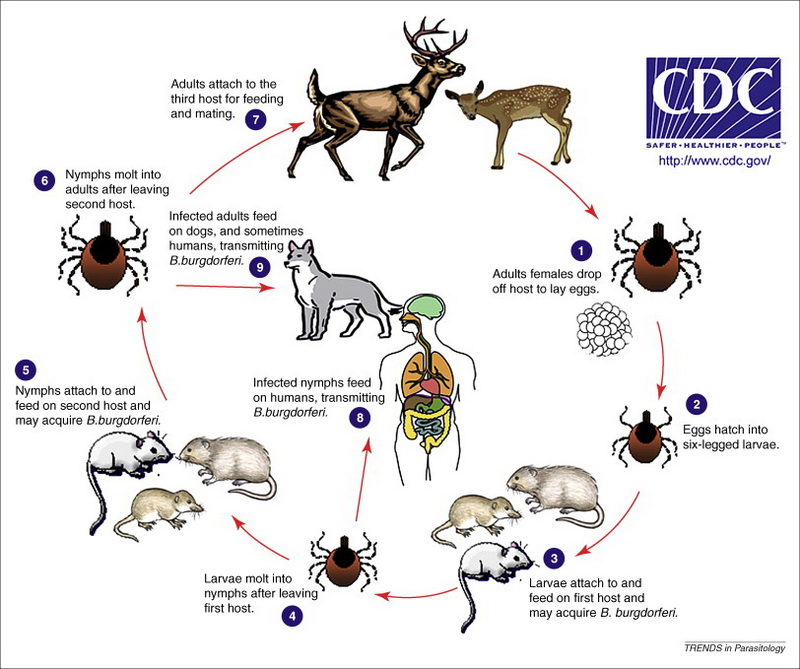
\includegraphics[width=\linewidth]{cycle-of-lyme-disease.jpg}
  \caption{Cycle of Lyme disease. \textit{B. burgdorferi} is the bacteria that causes Lyme disease.
  there are multiple times in a tick's life cycle where it can contract and potentially spread the disease.}
  \label{fig:cycle_lyme}
\end{figure}

Lyme disease is caused by the \textit{B. burgdorferi} bacteria in blacklegged ticks in the U.S
and can cause rash, fever, body aches, facial paralysis, and arthritis \cite{cdc_faq}.
Figure \ref{fig:cycle_lyme} shows the life cycle of Lyme disease.
There are many points in the tick's life cycle where it attaches to a host and potentially contract the \textit{B. burgdorferi} bacteria.
Rodents and deer are key to the tick's life cycle.

Compartmental models are typically used in infectious disease modeling to get the overall system dynamics of a disease.
The some of the homogeneous limitations in these models can be addressed by using patch models,
where compartments are broken up into smaller 'patches', and separate flow rates are determined between patches.

Significant associations between Lyme incidence and underlying geology, elevation, slope, and soil type, favoring coniferous non-herbaceous growth, are well known in the literature \cite{glass1995}.
However, among environmental factors, the presence of edge-habitats,
where deer prefer to dwell, seems to be the most consequential driver of the disease.

Forest fragmentation is strongly associated with a reduction of species diversity.
In the case of ticks and Lyme disease, 
when species (rodent) diversity decreases,
the probability of the remaining species becoming into contact with ticks increases.

\section{Problem Description}

\begin{figure}[hb!]
  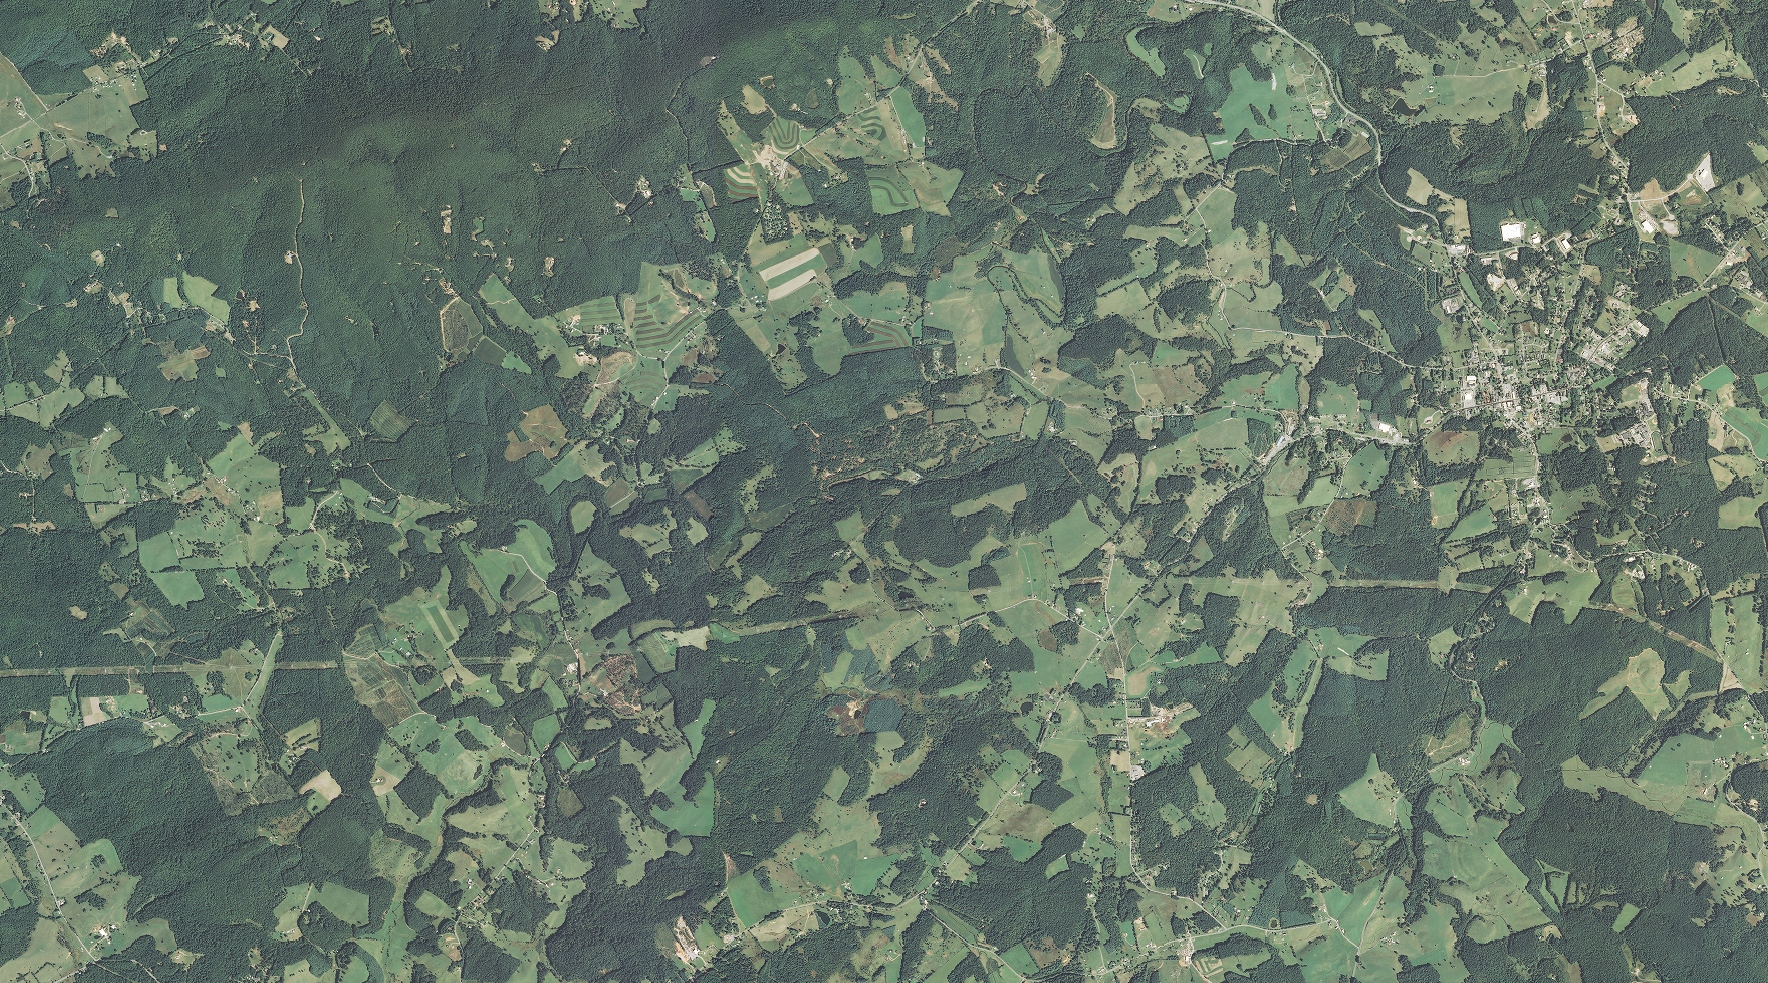
\includegraphics[width=\linewidth]{floyd.jpg}
  \caption{Map of Floyd, VA in 1x1 meter resolution}
  \label{fig:floyd}
\end{figure}

Our goal was to find and classify regions of forest in the town of Floyd, Virginia, and quantify forest fragmentation in order to model Lyme disease since it drives up tick and mice numbers. The existing 30 X 30 meter land cover data does not have resolution to allow us to identify small fragments and weirdly shaped edges. 

\section{Previous Work}

Previous classification and analysis was performed using ENVI by Harris Geospatial Solutions.
The Raw RGB data of the image was fed though three different classification algorithms within ENVI

\begin{enumerate}
\item Maximum Likelihood
\item Minimum Distance
\item Spectral Angle Mapper
\end{enumerate}

\subsection{Maximum Likelihood}

Maximum likelihood classification assigns each pixel to the corresponding class that has the highest probability \cite{envi_ml}.
ENVI's maximum likelihood calculates the discriminant functions for each pixel in the image:

\begin{equation}
g_i(x) = \ln p(w_i) - \frac{1}{2} ln \left|\sum_i\right| - \frac{1}{2}(x - m_i)^T \sum_i^{-1}(x - m_i)
\end{equation}

where \cite{envi_ml}:

\begin{itemize}
\item $i$ = class
\item $x$ = n-dimensional data (where n is the number of bands)
\item $p(w_i)$ = probability that class $w_i$ occurs in the image and is assumed the same for all classes
%\item $\left|\sum_i\right|$ = determinant of the covariance matrix of the data in class $ω_i$
%\item $\sum_i^{-1}$ = its inverse matrix
\item $\sum_i$ = covariance matrix of the data in class $ω_i$
\item $m_i$ = mean vector
\end{itemize}

\begin{figure}[ht!]
  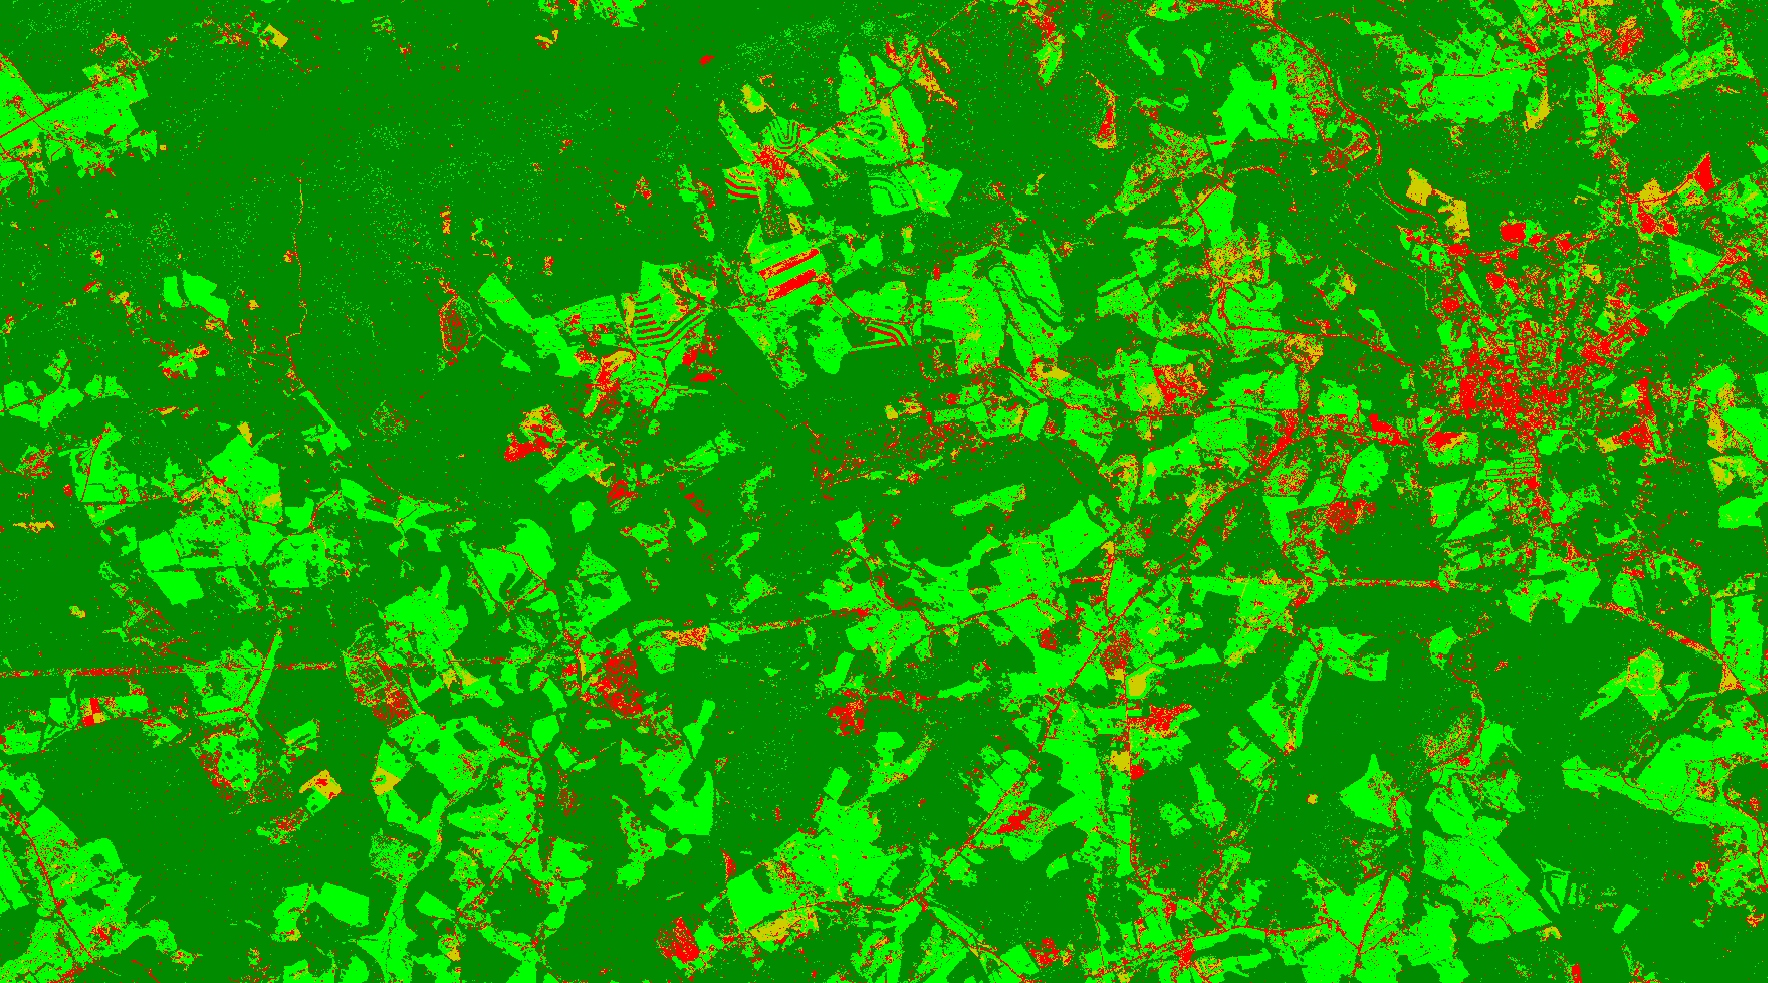
\includegraphics[width=\linewidth]{floyd_ML.jpg}
  \caption{Classification using Maximum Likelihood.
  Dark green are forest. Light green are fields, Red are urban areas, and tan are bare earth (e.g., dirt, rocks)}
  \label{fig:ml}
\end{figure}

\subsection{Minimum Distance}

Minimum distance calculates the Euclidean distance from each unknown pixel to the mean vector for each class \cite{envi_md} and classifies based on the minimum distance calculated.
This technique is similar to k-nearest neighbors.

\begin{figure}[ht!]
  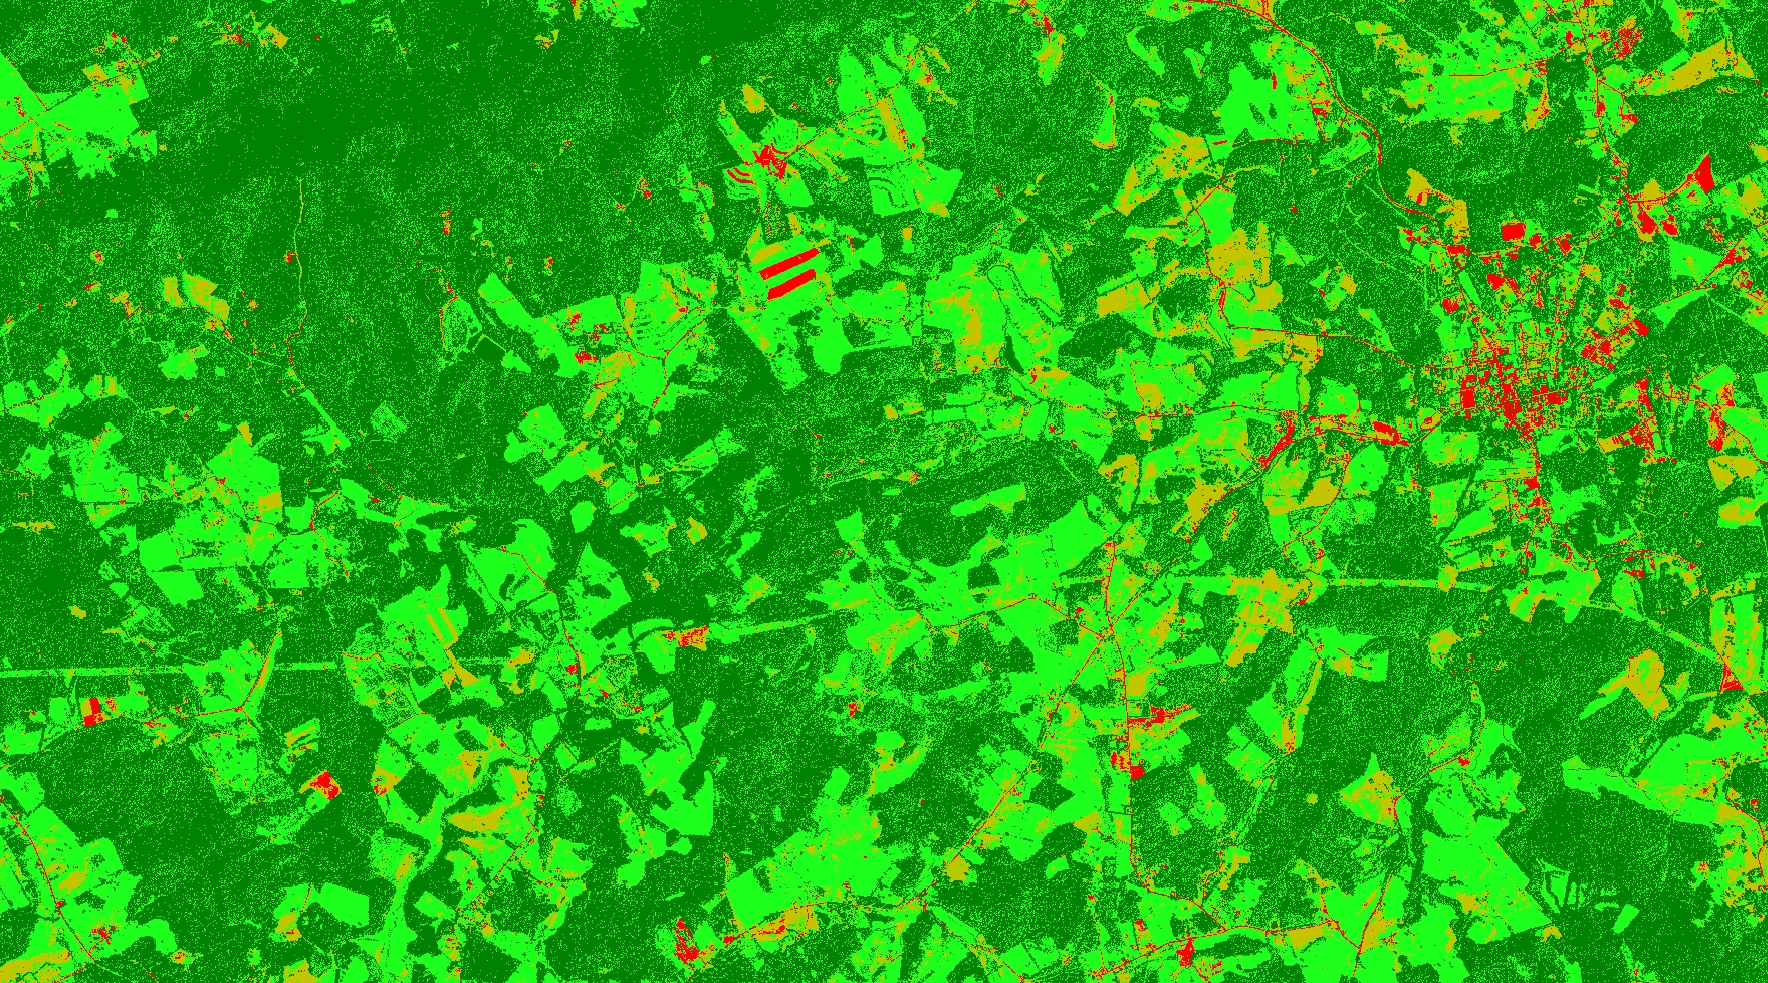
\includegraphics[width=\linewidth]{floyd_md.jpg}
  \caption{Classification using Minimum Distance.
  Dark green are forest. Light green are fields, Red are urban areas, and tan are bare earth (e.g., dirt, rocks)}
  \label{fig:md}
 \end{figure}

\subsection{Spectral Angle Mapper}

Spectral Angle Mapper (SAM) represents spectral information as an n-Dimensional vector and compares this vector to the reference spectra.
The angle created between these vectors determine the classification.
Angles greater than the maximum angle threshold are not classified \cite{envi_sam}.
This technique is similar to cosine similarity.

\begin{figure}[ht!]
  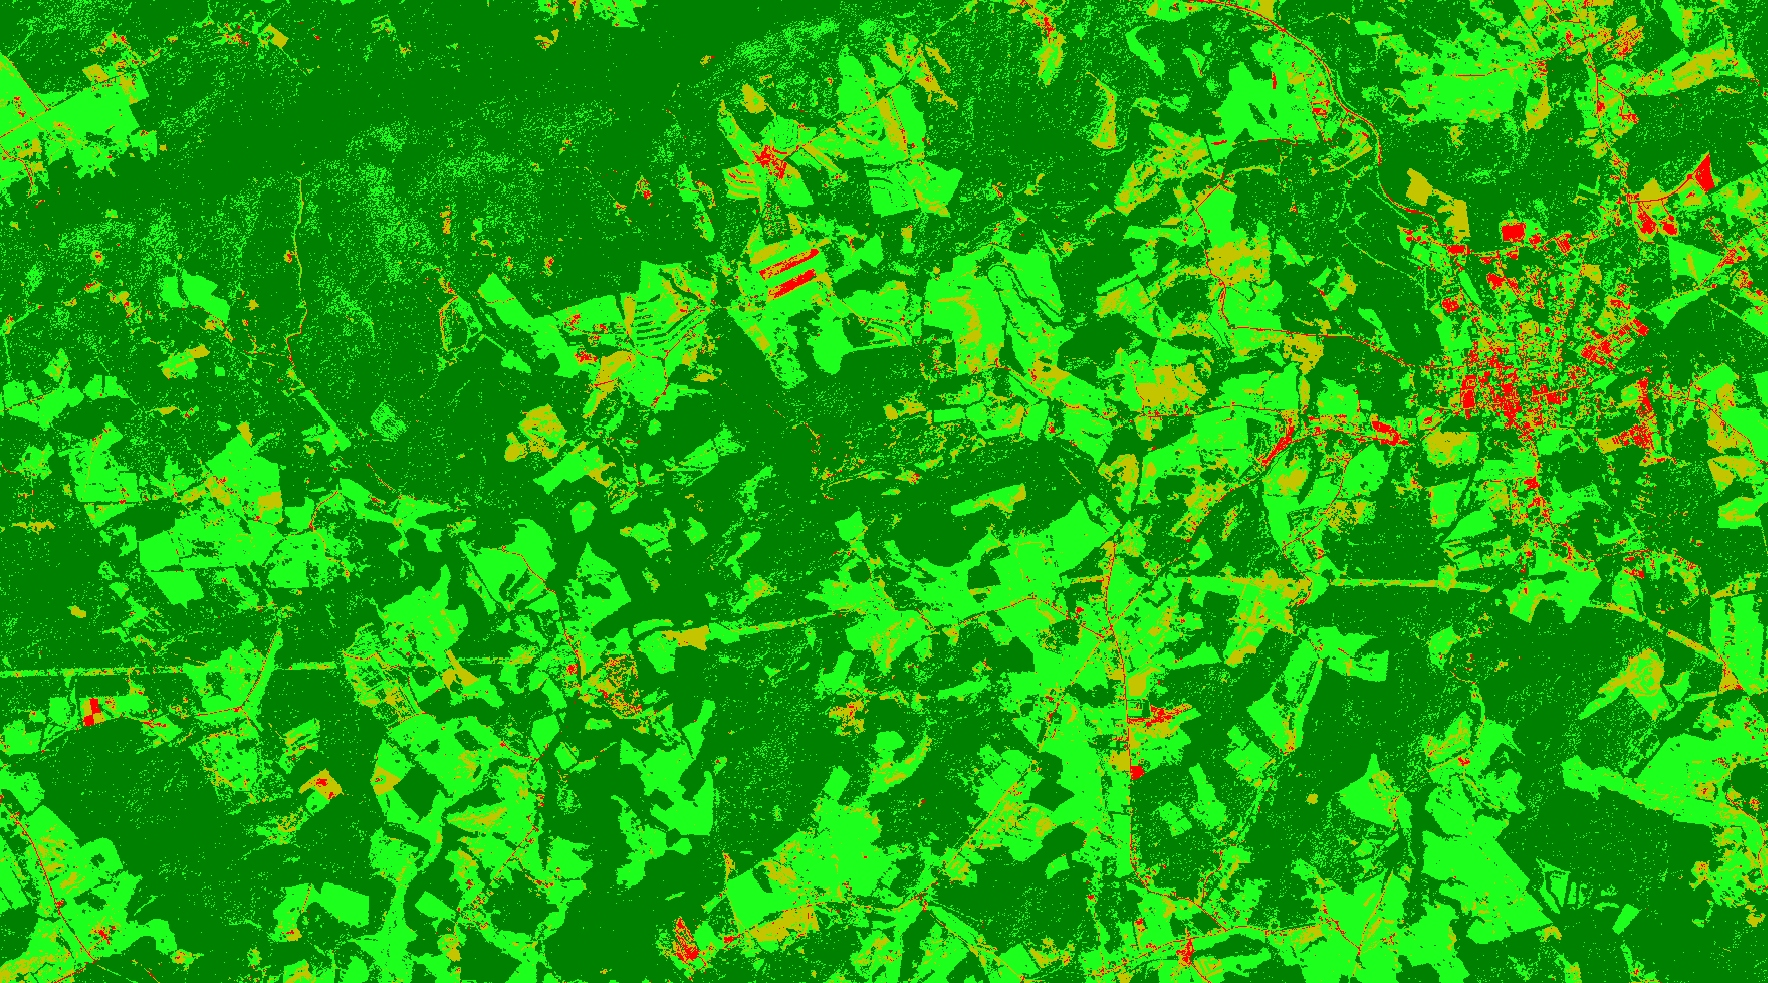
\includegraphics[width=\linewidth]{floyd_sam.jpg}
  \caption{Classification using Spectral Angle Mapper.
  Dark green are forest. Light green are fields, Red are urban areas, and tan are bare earth (e.g., dirt, rocks)}
  \label{fig:sam}
\end{figure}

\subsection{Other approaches}

Apart from these approaches, other previous approaches included multinomial logistic regression and SVM.
However, upon visual inspection of the classifications,
they were not performing well, per Pyrros Telionis, MPH (Network Dynamics and Simulation Science Laboratory),
to be reported.

\section{Our Approach}
Based on our survey of existing state of the art land cover classification methods, we realized that pixel based approaches, solely function on the color information present in a pixel of satellite or aerial image. These techniques do not take into consideration, the neighborhood information for making predictions. We feel that a color of pixels neighbors can help with the classification task. Since, the problem of detecting regions of forests does not mandate pixel by pixel classification, we can perform forest region classification on a block of pixels at a time. This assumption, transforms the problem into a computer vision task, where a block of pixels can be thought of as an image and a binary image classification algorithm, can either label the block as a forest region ($class-0$) or a non-forest region ($class-1$), hence detecting blocks of forests in a large aerial image. A block has a width and length in terms pixels and, we particularly look at block sizes of 100 X 100, 50 X 50 and 10 X 10 pixels. Figure \ref{fig:approach} summarizes our approach (sampling, training and prediction processes). 
\begin{figure*}
\centering
  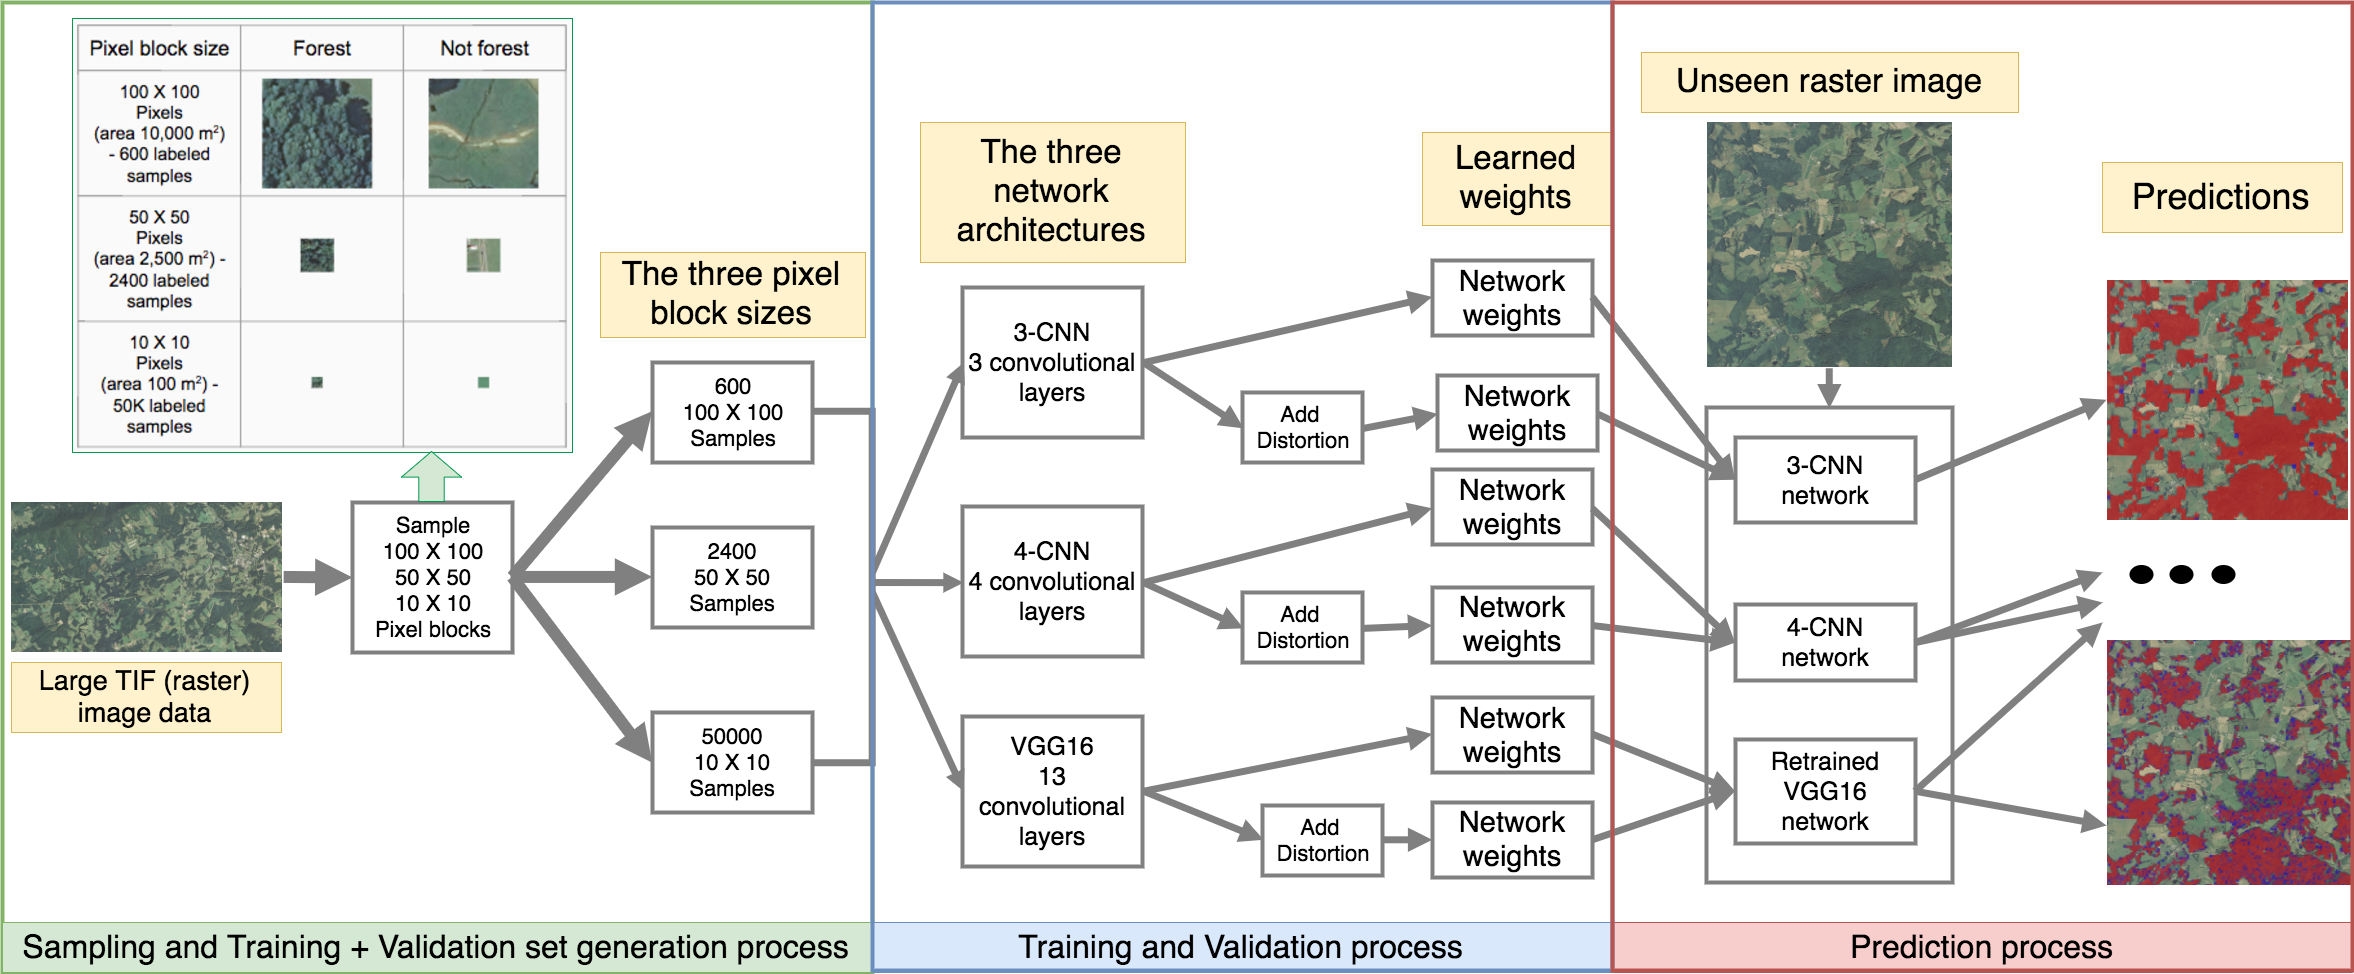
\includegraphics[width=\linewidth]{approach.png}
  \caption{Modeling and prediction approach.}
  \label{fig:approach}
\end{figure*}

Convolutional neural networks (CNNs) are feed-forward artificial neural networks, inspired by biological processes and can be thought of as variations of multilayer perceptrons, designed to use minimal amounts of preprocessing. They consist of multiple layers of receptive fields each of which are a small collection of neurons that process portions of an input image. The outputs of these collections are then ``tiled'' in such a way that their input regions overlap, and a higher-resolution representation of the original image is obtained. This is process is repeated for every layer \cite{wiki:cnn}. Deep convolutional neural networks, are the state of the art image classification algorithms, which have been shown to perform extremely well during image classification tasks \cite{krizhevsky2012imagenet}. In this study, we experiment using three deep neural network architectures, each with a different number of convolution layers. These three architectures are:
\begin{enumerate}
\item \textbf{[3-CNN]}: Having a total of 15 layers including 3 convolutional layers and 2 fully connected layers.
\item \textbf{[4-CNN]}: Having a total of 22 layers including 4 convolutional layers and 6 fully connected layers.
\item \textbf{[Retrained VGG16]}: Having a total of 41 layers including 13 convolutional layers and 3 fully connected layers. The model was developed by Visual Geometry Group, University of Oxford \cite{Simonyan14c}. We performed transfer learning \cite{Oquab_2014_CVPR} here, by replacing the top layer of the VGG16 model, so that it can perform binary image classification, and the resulting model was retrained on our image data.
\end{enumerate}
Next, we discuss the data pre-processing steps we used in this work.
\subsection{Pre-processing}
To generate the training set for each of the window sizes, we began by randomly extracting 8000, 100 X 100 pixel raster images from the large data file. Since, majority of the land cover in the image was forests, most of the sampled images ($\approx 7000$) only contained forests. But, in order to create a balanced training and evaluation dataset, we need to have an equal number of positive and negative samples. Due to the sparsity of non-forest samples we ended up manually labeling 600 of these samples, half of which were forests and half were non-forests. This served as the dataset for all our experiments that use an input image size of 100 X 100 pixels. A large image containing forests, can be split into multiple small images, which also contain forests and this. We use this strategy to generate samples of smaller dimensions (50 X 50 and 10 X 10 pixels) from the 100 X 100 pixel samples. So, we split each of the 100 X 100 pixel images into 4, 50 X 50 pixel images, resulting in a total of 2400 samples (1200 samples for each class). This served as the dataset for all our experiments which use an input image size of 50 X 50 pixels. Next, we split 2000 of these 50 X 50 pixel images into 10 X 10 pixel images, resulting in a total of 50000 samples (25000 samples for each class). This served as the dataset for all our experiments which use an input image size of 10 X 10 pixels. Also, since the objective of this exercise is to ultimately use the model to make predictions on unseen data, a 5500 X 5500 pixel portion of the large aerial image was excluded from the sampling process. The final predictions, which are presented in the results section, were made on this particular portion of the aerial image. Next we discuss the various experiments that we did using the three deep convolutional network architectures, i.e. \textbf{3-CNN}, \textbf{4-CNN} and \textbf{VGG16}.  
\subsection{Experiments}
We performed the following experiments:
\begin{enumerate}
\item The first set of experiments were done with the 600 samples each of size 100 X 100 pixel, split in the ratio of 2:1 for training and validation. The three convolutional layers present in \textbf{3-CNN} network, had filter depths of 32, 64 and 64 respectively each followed by a Relu activation. We subsequently added one more convolutional layer with a filter depth of 64, along with 4 dense layers to this model to obtain the \textbf{4-CNN} network. We executed 50 training epochs, in each epoch a total of 25 training iterations were executed, and 16 training samples were propagated through the networks in one iteration (i.e. the batch size was 16 samples).  
\item The second set of experiments were done with the 2400, 50 X 50 pixel samples, 2000 samples were set aside for training and the rest were used for validation. Once again we used the \textbf{3-CNN} and \textbf{4-CNN} networks described above for this experiment. We again executed 50 training epochs with 125 training iterations per epoch and a batch size of 16. 
\item The third set of experiments were done with the 50000, 10 X 10 pixel samples, 40000 samples were set aside for training and the rest were used for validation. Once again we used the \textbf{3-CNN} and \textbf{4-CNN} networks described previously for this experiment. We executed this for 50 training epochs with 2500 training iterations per epoch and a batch size of 16.
\item The fourth set of experiments were done with each of the three datasets (i.e. 100 X 100, 50 X 50 and 10 X 10 pixel samples), using the \textbf{4-CNN} network with distortions added to the input images while training. The objective was to understand the impact of distortions on model performance. We used the following 5 image distortions:
 \begin{enumerate}
 \item \textbf{Shear:} Apply shear mapping to the image in the range of $[0, 0.2]$ radians in the counter-clockwise direction.
 \item \textbf{Zoom:} Apply zoom to the image in the range of $[0.8, 1.2]$.
 \item \textbf{Horizontal flip: } Flip the image horizontally.
 \item \textbf{Vertical flip: } Flip the image vertically.
 \item \textbf{Rotation:} Apply rotation to the image in the range$[0,360]$ degrees.
 \end{enumerate}
These distortions were randomly applied to the input image samples, before propagating them through the network, in the training phase. Such distortions are often used to improve the results of image training and are particularly useful when the training data is small and these. In a way, distortions expand the effective size of the training data by adding variations of the same images. Adding distortions also tend to help the networks learn to cope with distorted versions of images, which might occur in the real world.  
\item The last set of experiments were done with the 100 X 100 and 50 X 50 pixel datasets but in this case we retrained the \textbf{VGG16} network instead of building and training a network from scratch. We also applied the five distortions discussed above, during the training phase. 
\end{enumerate}
After each of these experiments, we saved the weights learned by the networks, for later use (prediction). We also saved the learning history (change in training accuracy, training loss, validation accuracy and validation loss) and plotted these for each of the experiments. After all the training experiments were completed, we used the saved weights of the models to make predictions on an image which was not used during the training and validation steps. These predictions on the previously unseen image along with other results are presented in the next section.   
\section{Results}
We present the output of the above experiments in terms of model prediction, loss and some model visualizations. For prediction and model comparison purposes a 5500 by 5500 pixel image, shown in figure \ref{fig:55}, was taken out from the large image and was sliced into smaller blocks according to the window size used in the model. As an example, for 3-CNN 100x100 case, the image was split into 3025 smaller windows and prediction was done on each of them individually, and at the end predictions were stitched together and was added as a layer on the top of the original image. 

\begin{figure}[ht!]
\centering
  \includegraphics[width=0.8\linewidth]{AerialFloyd_cropped.jpg}
  \caption{The 55K X 55K pixel image on which the predictions were made.}
  \label{fig:55}
\end{figure}

%\subsection{100x100}
It is important to note that the predictions had to be done on an unlabeled image, i.e. the prediction quality perhaps could only be judged by visual inspection of the results. If an image window was classified as forest (probability of being in forest class $>$ 0.5) by the deep net model, then that window was represented as a colored box where the color could vary from red to blue, red denoting very high probability of belonging to forest class, and blue denoting  probabilities close to 0.5. We also plot the binary-cross entropy loss for each model over epochs. 

Decreasing window size did improve the overall prediction accuracy on the unlabeled image (fig \ref{fig:predict_100}, \ref{fig:predict_50}, \ref{fig:predict_10}). In almost all the cases forests were being predicted with very high probability, but some of the farm lands and few surrounding areas were also being classified as forest when a bigger window size was used. As we decrease the window size that problem was partially addressed, but in order to have more robust model new convolution and dense layers were added to the base model and distortions were introduced in the training data. That improved the prediction accuracy as well as solved the problem of over fitting. We believed that the 10x10 window size was sufficient to accurately draw a border between forest and non forest. The prediction probability i.e. probability of being classified as forest were mostly close to 1, except few cases, such as near farm lands enclosed by forests, where the model was not very confident about predicted label (encoded as blue boxes in fig \ref{fig:predict_100}, \ref{fig:predict_50}, \ref{fig:predict_10}). The prediction by VGG16 model was more conservative than the other models in terms of detecting forest lands. Two different window sizes were tried on VGG16 model. We had no reason to expect better results by VGG16 than our models, since VGG16 had been trained with object images and for different purpose. But it was still able to provide a reasonable output after retraining only the last layer.

The loss curves (fig \ref{fig:loss_100}, \ref{fig:loss_50}, \ref{fig:loss_10}, \ref{fig:loss_VGG}, table \ref{tab:summary}) were not particularly encouraging, as the validation loss did not monotonically decrease in all of our models, although the training error decreased over time. On the contrary VGG16 showed a decent learning improvement over time. We also tried to plot class activation maps \cite{zhou2015cnnlocalization} for 100x100 case since cam figures for small windows were not visually understandable due to its size. Class activation maps show heatmap of the activation functions for different class labels. In each of the 3 plots in fig \ref{fig:cam} the first column panel shows original image, the second panel shows the activation map for forest label and the last panel show the activation map for non forest label. As the forest and non forest were encoded as 0 and 1 respectively in NN models, we see large red areas on the non-forest panel which detects the non forest as 1 and in the second panel we see only few spots where the activation function was actually active (i.e. detecting as non-forest).

\begin{table*}[htbp!]
\centering
\caption{Models summary}
  \label{tab:summary} 
\begin{tabular}{@{\extracolsep{5pt}} llcccc} 
\\[-1.8ex]\hline 
\hline \\[-1.8ex] 
 & Model & Training accuracy & Validation accuracy & Training loss & Validation loss \\ 
\hline \\[-1.8ex] 
1 & 100x100 3cnn & $1$ & $0.957$ & $0.0004$ & $0.372$ \\ 
2 & 100x100 4cnn & $1$ & $0.984$ & $0.001$ & $0.134$ \\ 
3 & 100x100 4cnn with distort & $0.998$ & $0.978$ & $0.025$ & $0.149$ \\ 
4 & 50x50 3cnn & $0.983$ & $0.992$ & $0.086$ & $0.075$ \\ 
5 & 50x50 4cnn & $0.976$ & $0.978$ & $0.090$ & $0.093$ \\ 
6 & 50x50 4cnn with distort & $0.976$ & $0.978$ & $0.095$ & $0.083$ \\ 
7 & 10x10 3cnn & $0.944$ & $0.959$ & $0.228$ & $0.138$ \\ 
8 & 10x10 3cnn with distort & $0.936$ & $0.959$ & $0.482$ & $0.221$ \\ 
9 & vgg16/100x100 with distort & $0.990$ & $0.964$ & $0.062$ & $0.130$ \\ 
10 & vgg16/50x50 with distort & $0.953$ & $0.962$ & $0.148$ & $0.108$ \\ 
\hline \\[-1.8ex] 
\end{tabular}
\end{table*}

%%% prediction plot

\begin{figure*}[ht!]
\centering
  \includegraphics[width=0.3\linewidth]{3cnn_100.jpg}
  \includegraphics[width=0.3\linewidth]{4cnn_100.jpg}
  \includegraphics[width=0.3\linewidth]{4cnnwithdistort_100.jpg}
  \caption{Forest prediction using image window of 100x100 pixels by 3-CNN, 4-CNN and 4-CNN with distortion respectively from left to right.}
  \label{fig:predict_100}
\end{figure*}
\begin{figure*}[ht!]
\centering
  \includegraphics[width=0.3\linewidth]{3cnn_50.jpg}
  \includegraphics[width=0.3\linewidth]{4cnn_50.jpg}
  \includegraphics[width=0.3\linewidth]{4cnnwithdistort_50.jpg}
  \caption{Forest prediction using image window of 50x50 pixels by 3-CNN, 4-CNN and 4-CNN with distortion respectively from left to right.}
  \label{fig:predict_50}
\end{figure*}
\begin{figure*}[ht!]
\centering
  \includegraphics[width=0.3\linewidth]{3cnn_10.jpg}
  \includegraphics[width=0.3\linewidth]{3cnnwithdistort_10.jpg}
  \caption{Forest prediction using image window of 10x10 pixels by 3-CNN and 3-CNN with distortion respectively from left to right.}
  \label{fig:predict_10}
\end{figure*}
\begin{figure*}[ht!]
\centering
  \includegraphics[width=0.3\linewidth]{50withdistort.jpg}
  \includegraphics[width=0.3\linewidth]{100withdistort.jpg}
  \caption{Forest prediction using image window of 50x50 pixels and 100x100 pixel by retrained VGG16 respectively from left to right.}
  \label{fig:predict_VGG}
\end{figure*}


%%% loss plots

\begin{figure*}[ht!]
\centering
  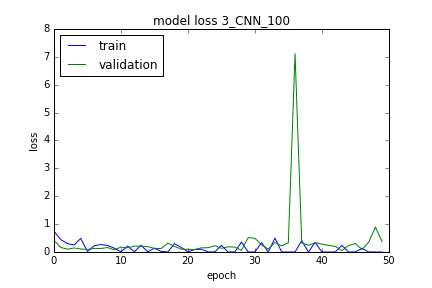
\includegraphics[width=0.3\linewidth]{3_CNN_100_loss.png}
  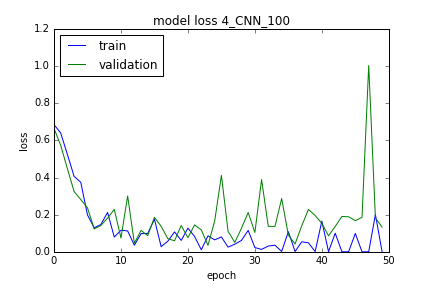
\includegraphics[width=0.3\linewidth]{4_CNN_100_loss.png}
  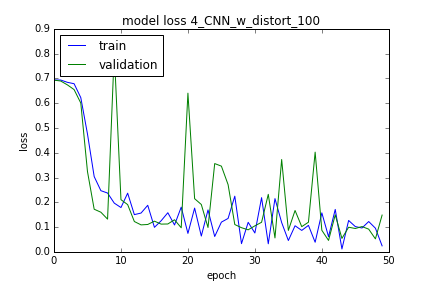
\includegraphics[width=0.3\linewidth]{4_CNN_w_distort_100_loss.png}
  \caption{Plot of loss over epoch for the model using image window of 100x100 pixels by 3-CNN, 4-CNN and 4-CNN with distortion respectively from left to right.}
  \label{fig:loss_100}
\end{figure*}
\begin{figure*}[ht!]
\centering
  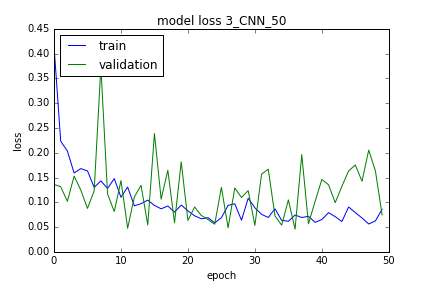
\includegraphics[width=0.3\linewidth]{3_CNN_50_loss.png}
  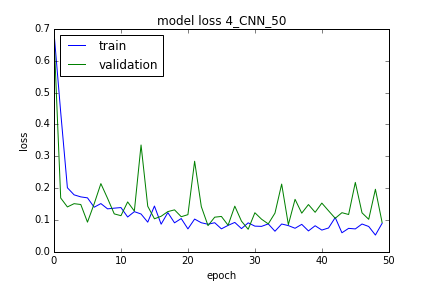
\includegraphics[width=0.3\linewidth]{4_CNN_50_loss.png}
  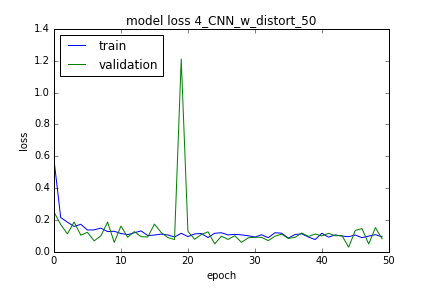
\includegraphics[width=0.3\linewidth]{4_CNN_w_distort_50_loss.png}
  \caption{Plot of loss over epoch for the model using image window of 50x50 pixels by 3-CNN, 4-CNN and 4-CNN with distortion respectively from left to right.}
  \label{fig:loss_50}
\end{figure*}
\begin{figure*}[htbp!]
\centering
  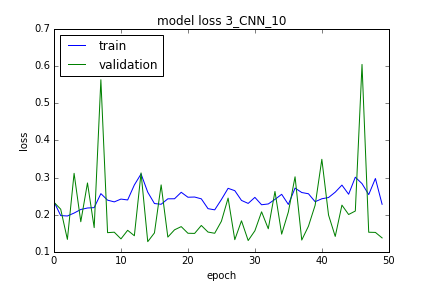
\includegraphics[width=0.3\linewidth]{3_CNN_10_loss.png}
  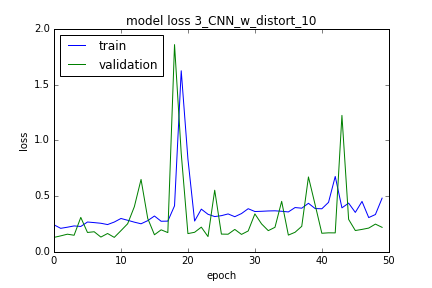
\includegraphics[width=0.3\linewidth]{3_CNN_w_distort_10_loss.png}
%  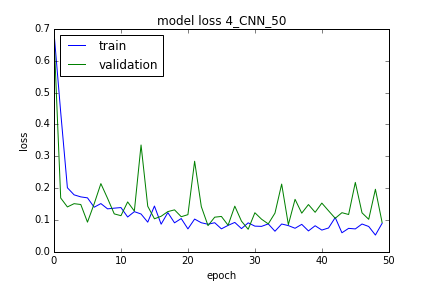
\includegraphics[width=0.3\linewidth]{4_CNN_50_loss.png}
%  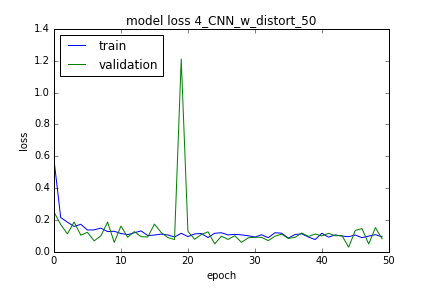
\includegraphics[width=0.3\linewidth]{4_CNN_w_distort_50_loss.png}
  \caption{Plot of loss over epoch for the model using image window of 10x10 pixels by 3-CNN and 3-CNN with distortion respectively from left to right.}
  \label{fig:loss_10}
\end{figure*}
\begin{figure*}[htbp!]
\centering
  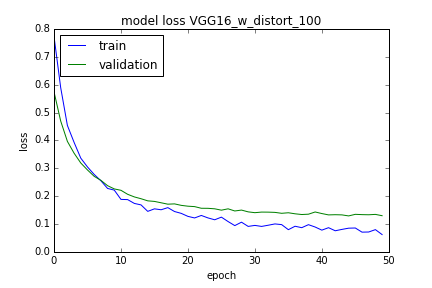
\includegraphics[width=0.3\linewidth]{VGG16_w_distort_100_loss.png}
  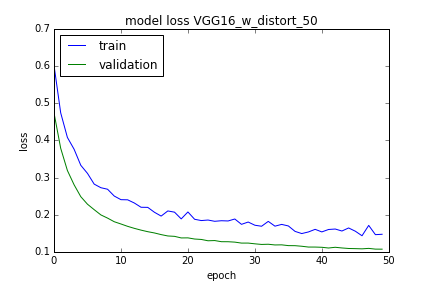
\includegraphics[width=0.3\linewidth]{VGG16_w_distort_50_loss.png}
  \caption{Plot of loss over epoch for the model using image window of 100x100 pixels  and 50x50 by VGG16 with distortion respectively from left to right.}
  \label{fig:loss_VGG}
\end{figure*}

% \begin{figure}
%   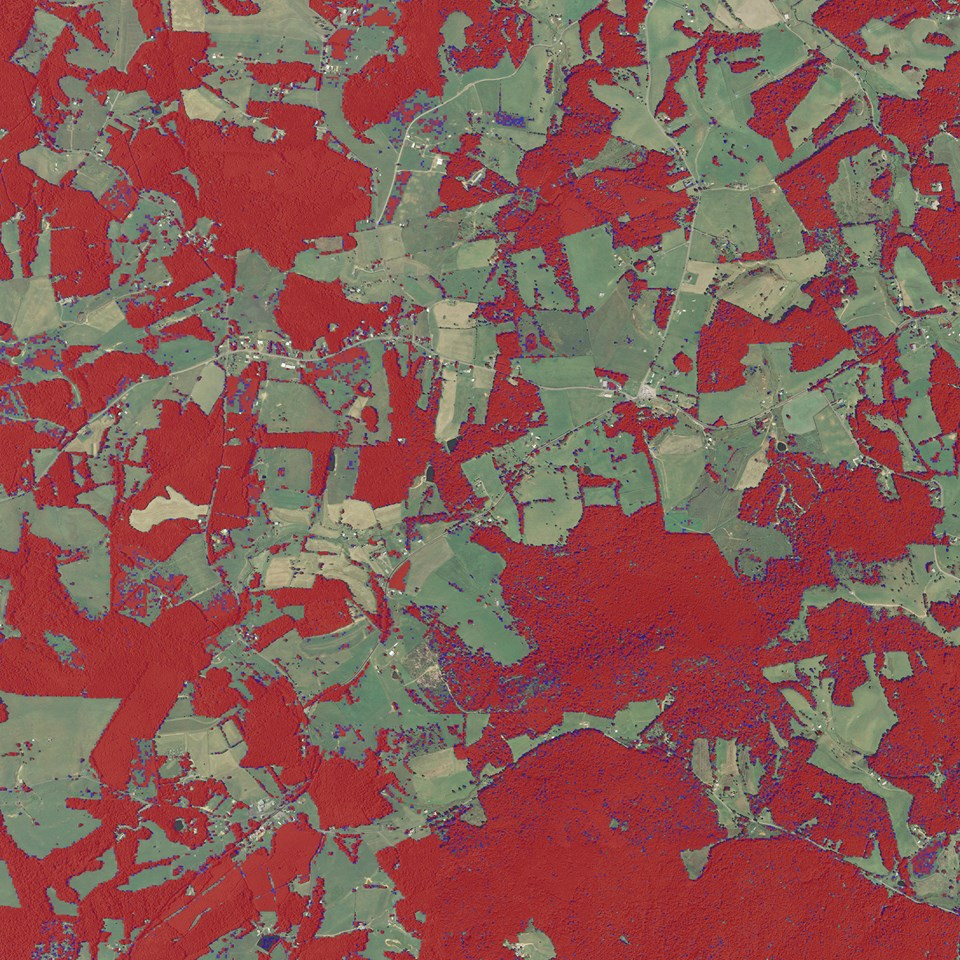
\includegraphics[width=\linewidth]{cnn_results_10x10.jpg}
%   \caption{CNN}
%   \label{fig:10result}
% \end{figure}

% \begin{figure}
%   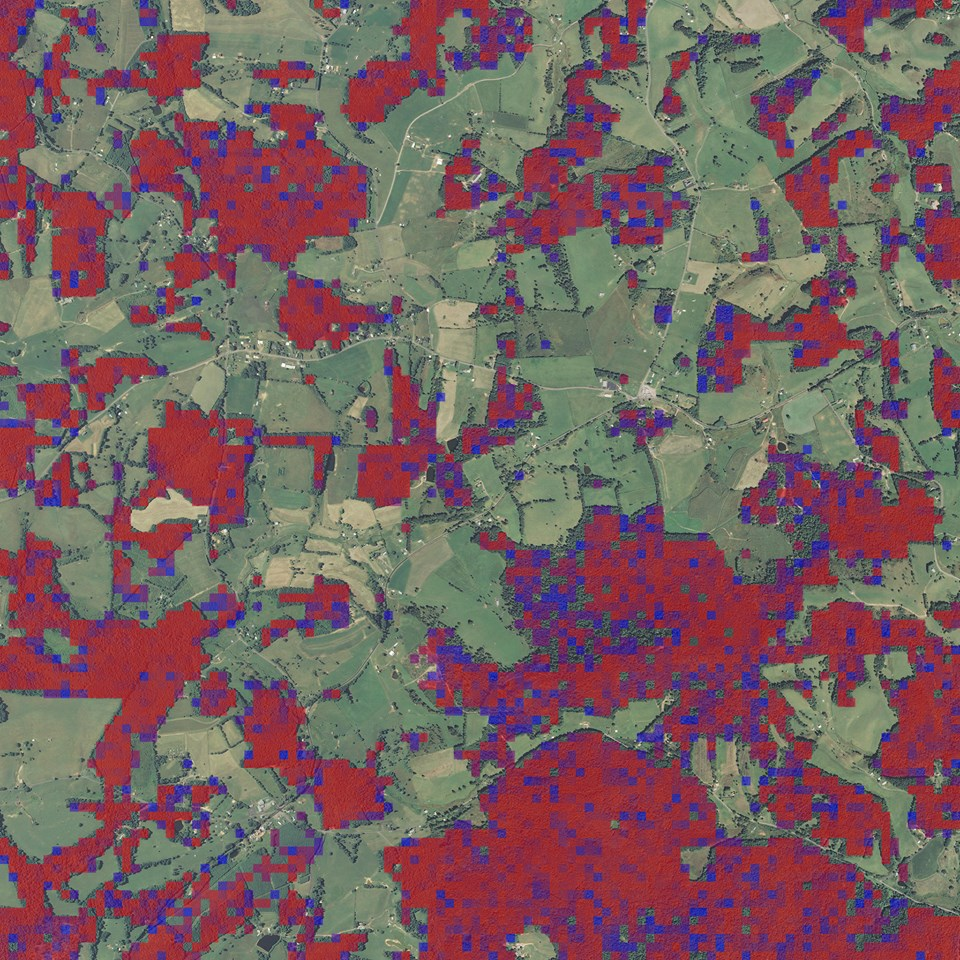
\includegraphics[width=\linewidth]{transfer_learning_results.jpg}
%   \caption{xfer learning}
%   \label{fig:vgg16result}
% \end{figure}


\begin{figure*}[htbp!]
\centering
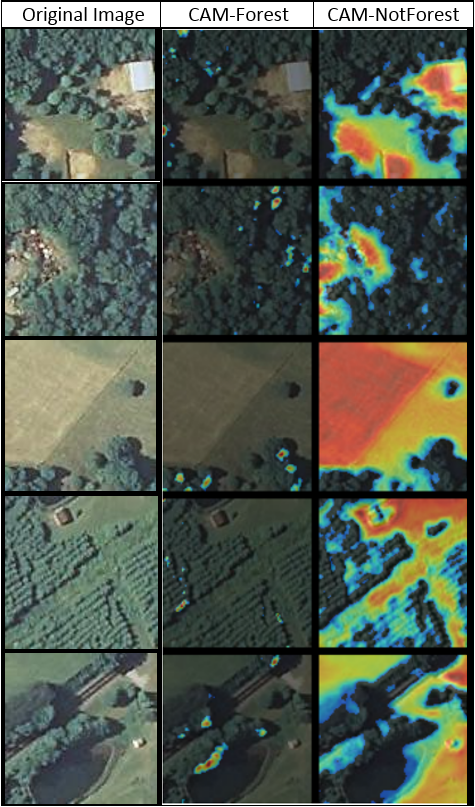
\includegraphics[width=0.3\linewidth]{3cnn_cam.png}
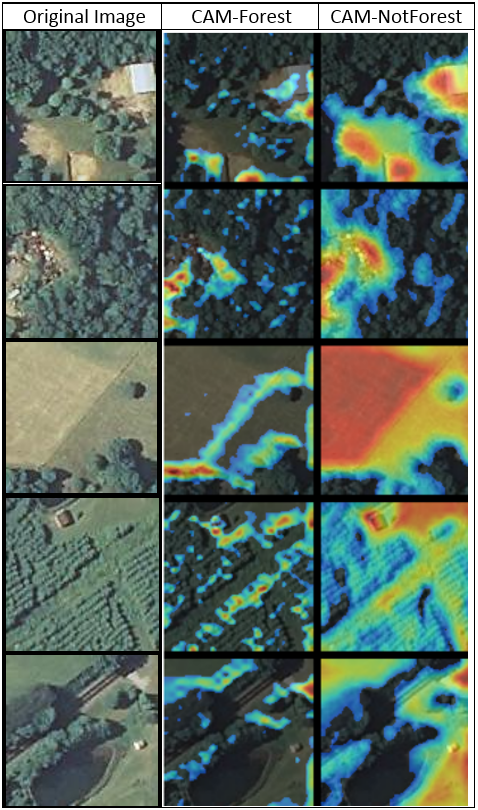
\includegraphics[width=0.3\linewidth]{4cnn_cam.png}
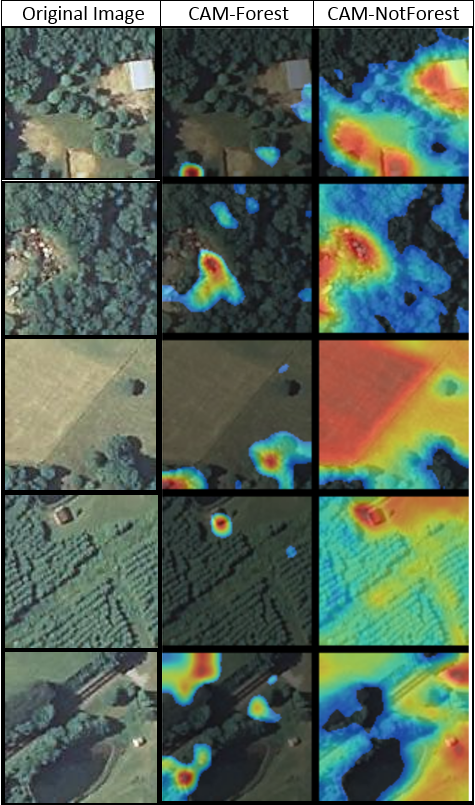
\includegraphics[width=0.3\linewidth]{4cnn_distort_cam.png}
  \caption{Class activation map (CAM) for 3-CNN, 4-CNN, 4-CNN with distortion models using 100x100 window size (from left to right respectively).}
  \label{fig:cam}
\end{figure*}

\section{Challenges}
Throughout this study, we were faced with various technical and domain challenges, we list some of these below:
\begin{enumerate}
\item \textbf{Large image data:} Due to the prohibitively large size of the initial image (5.67 GB) we had to use GIS software Q-GIS \cite{QGIS_software}, to extract the initial 100 X 100 pixel raster samples. 
\item \textbf{Difficult to label samples:} The number of initial samples that were extracted was 8000, sifting through these to obtain good samples specially for the non-forests class was a mammoth task. Also, many a times some portion of 100 X 100 samples, had forest cover, it is difficult if not impossible, to provide an exact label to such samples. We generally followed a majority rule while labeling such samples, i.e. if more than $50\%$ of a sample has forest cover, we label it as a forest, if there is less than $50\%$ forest cover, we label it as non-forest, and discard samples which have almost $50\%$ forest cover. For some sample images, it was difficult even for a human being to say with confidence, whether the sample is a forest or not (local water bodies, like ponds and small lakes, acquire a green hue due to surface algae, this along with the surface reflections, make them indistinguishable from forests.)  
\item \textbf{Challenges while predicting:} After the training process, predictions had to be made on large images. These images required to be processed into small blocks of pixels (100X100, 50X50 and 10X10) for ingestion into the trained neural network, so as to produce a class label and prediction probability. After the prediction step these labels had to be visualized over the respective blocks of pixels in the original image. This was highly resource intensive (both in terms of memory and processing).
\item \textbf{Challenges after predicting:} There is no gold standard, labeled dataset available for the problem we are trying to solve, and predictions made by the models on previously unseen and unlabeled images can only be evaluated visually by a human being. Based on our observations and those of the domain experts, our technique seems to do well on the current dataset, but a quantitative metric (say accuracy) cannot be obtained for unlabeled data. The challenge of labeling new data makes this problem much harder.      
\end{enumerate}

\section{Conclusion and Future Work}
In this paper, we discussed an approach that takes into account, pixel neighborhood information instead of individual pixel color information which is used in traditional land cover detection algorithms. We discussed this problem as an image classification challenge and used state of the art image classification techniques (deep convolutional neural networks) for this problem. The initial results presented in this work, seem to be promising and these can be used to find edge regions of forests.
This will allow researchers to study and find habitats and quantify forest fragmentation. As mentioned in the introduction,
Rodents and deer inhabit these edge forest regions,
and forest fragmentation contributes to a decrease in biodiversity, which are all contributing factors to the motivation for this effort which is modeling Lyme disease.\\

Other than the experiments presented in this paper, we also ran experiments using larger sample sizes $\approx 6000$ samples for the 100 X 100 case, but these didn't give substantially better predictions on the unseen image data as compared to the case when we only used 600 samples.

\section{Acknowledgements}
We would like to thank Pyrros Telionis, MPH for providing us the high resolution aerial image data used in this study. He also provided us with some of the results presented in the previous work section. We would also like to thank Prof. Bert Huang for introducing us to the area of deep learning, convolutional neural networks and transfer learning.

\newpage

\bibliographystyle{abbrv}
\bibliography{references}  % sigproc.bib is the name of the Bibliography in this case
% You must have a proper ".bib" file
%  and remember to run:
%latex bibtex latex latex
% to resolve all references
%
% ACM needs 'a single self-contained file'!
%
\end{document}

